\documentclass[a4paper,10.0pt,twoside]{npr}

\usepackage{multicol,graphicx,lastpage,footmisc,fancyhdr,paralist,
tabularx,array,booktabs,caption,multirow,upgreek,mathrsfs,gensymb,color}
\usepackage[fancyhdr,space,fntef,fontset=ubuntu]{ctex}
\usepackage{amssymb,bm,mathrsfs,bbm,amscd}
\usepackage{flushend,cuted}
\usepackage{refcount}
\usepackage{savesym}
\usepackage{textcomp}
\usepackage[tbtags]{amsmath}  %
\savesymbol{iint}
\usepackage{amstext} %数学宏包文本命令
\usepackage{balance} %版心底部对齐

\flushbottom      %版心底部对齐
\setcounter{section}{0}
\begin{document}
%\begin{CJK*}{GBK}{\song}{\wuhao}{\rm}

%___________________________________________________________________________________
\def\rd{{\rm d}}

\newcommand{\RM}{\ensuremath{\mathrm}}   %正体 既可用于文本模式也可用于数学模式
\newcommand{\dif}{\mathrm{d}}  %直立体d
\newcommand{\me}{\mathrm{e}}  %直立体e
\newcommand{\mi}{\mathrm{i}}  %直立体i
\newcommand{\mj}{\mathrm{j}}  %直立体j
\newcommand{\afrac}[2]{\dfrac{\,#1\,}{\,#2\,}}  %略长分数线
\newcommand{\nn}{\nonumber}  %公式无编号
\newcommand{\nt}{\noindent}
\newcommand{\OO}{~\text{。}}
\newcommand{\PP}{~\text{,}}
\newcommand{\OP}{~\text{;}}
\newcommand{\LT}{\left}
\newcommand{\RT}{\right}

%___________________________________________________________________________________

\balance
\fancypagestyle{myfoot}
{%
\fancyhf{}
\fancyhead[c]{\wuhao\song 高~等~核~物~理~实~验}
\renewcommand{\headrule}{\vskip 2pt
\hrule height0.4pt width\headwidth \vskip1pt
\hrule height0.4pt width\headwidth \vskip-1.8pt}
}%
\thispagestyle{myfoot}

%%%%%%%%%%%%%%%%%%%%%%%%%%%%%%%%%%%%%%%%%%%%%%%%%%%%%
%    奇偶页眉
%%%%%%%%%%%%%%%%%%%%%%%%%%%%%%%%%%%%%%%%%%%%%%%%%%%%%
\pagestyle{fancy}
\fancyhead{}
\fancyhead[ce]{\xiaowu\song \hspace{0.5em}高~等~核~物~理~实~验}
%\fancyhead[ro,le]{\xiaowuhao \hspace{0.5em}\textbf{\textperiodcentered}\;\thepage\;\textbf{\textperiodcentered}\hspace{0.5em}}
%\fancyhead[ce]{\xiaowu\song 粒~子~物~理~与~原~子~核~物~理~专~题~实~验}
%\fancyhead[re]{\xiaowu\song \hspace{0.5em}第\;31\;卷\hspace{0.5em}}
\fancyfoot[ce,co]{}
\renewcommand{\headrule}{\vskip 2pt
\hrule height0.4pt width\headwidth}


\setcounter{page}{001}%
\fancyhead[co]{\xiaowuhao\song  乔颢:用正比计数器测量X射线的吸收和特征谱}    %奇页页眉
\begin{center}
\title{%
\xiaoerhao \bf  %章标题为两行时改为 \exiaoer
用正比计数器测量X射线的吸收和特征谱\\[-5mm]}
\maketitle
\large \fs
乔颢$^{^1}$\\[2mm]

\xiaowu \song
1. 北京大学物理学院,海淀区 北京 100871;\\[4mm]

 
\footnotetext[0]{{\bf 作者简介:}~~\begin{minipage}[t][4.2mm]{149mm}\song
乔颢,E-mail: i@catofes.com
\end{minipage} }
%\footnotetext[0]{{\bf 通信作者:}\song ~~E-mail: xxx@xxx.xxx }%通信作者为第一作者时不要此项

\parbox{158mm} {
\zywu{\bf 摘要:}~~\fs
该实验使用正比计数器测量了不同材料在$^{238}$Pu的激发下,发射的X射线特征谱。并测量了铝对铜的X射线质量吸收系数为$54.0cm^2/g$。该探测器的能量分辨率为18.3\%。\\

{\bf 关键词:}~~\fs X射线, X射线特征谱, 正比计数器, 能量分辨率,质量吸收系数}\\
\end{center}
%%%%6.正文
\vspace{5mm}
%%%%6.正文
\setcounter{section}{0}
\begin{multicols}{2}
%----------------
%____________________________________________________________________________
%%%%以上请不要改动%%%%%%%%%%%%%%%%%%%%%%%%%%%%%%%%%%%%%%%%%%%%

\section{引言}    %1
\vspace*{-1mm}
\song\wuhao
X射线是一种电磁波,它的波长在100A到0.01A之间。当X射线入射到目标物质后,有可能将其内层电子打出,而外层电子跃迁会内层则会发射出新的X射线,也就是特征X射线谱。特征X射线在判别物质材料等方面有着广泛的应用。

本实验使用$^{238}$Pu发射出的X射线激发Zn、Cu、Ni等样品产生其特征X射线,并利用理论结果来确定待测样品的材料。同时也测量了X射线在铝中的吸收系数。通过本实验可以了解X射线与物质的相互作用以及其在物质中的吸收规律。

\section{实验原理}
\subsection{射线特征谱}
原子可以通过核衰变过程,即内转换和轨道电子俘获,也可以通过外部射线,如X射线、$\beta$射线、$\alpha$粒子或其他带电粒子与原子中电子相互作用产生内层电子空位,在电子跃迁时产生特征X射线。波尔理论指出电子跃迁时放出的光子具有一定的波长$\lambda$,它的能量是:
\begin{equation}
   h\mu = Z^2 \frac{2\pi^2m_0e^4}{h^2}(\frac{1}{n^2_1}-\frac{1}{n^2_2})
\end{equation}
因而根据特征X射线的能量,即可辨认出激发原子的原子序数。
\subsection{X射线的吸收}
当一束单色的X射线垂直射到吸收体上,通过吸收体后,其强度将减弱,即X射线的吸收。这一过程分为吸收和散射两部分。对于我们研究的铝,因为X射线的能量较低,所以光电吸收效应占优势,而康普顿散射则可以忽略。

理论上给出穿过厚度为t的成分均匀的吸收体,透射光子数满足:
\begin{equation}
   I(t)=I_0e^{-\mu t}
\end{equation}

\subsection{正比计数器}

正比计数器是一种气体放大器,其可以将入射例子产生的触及电离放大很多倍,而输出脉冲幅度仍保持着与最初电离事件数目成正比。正比管输出脉冲较大,而本身的噪声则很小,因而其在测量低能例子方面起着独特的作用。 

\section{实验内容和结果}

本次的实验仪器如图所示:
\begin{center}
   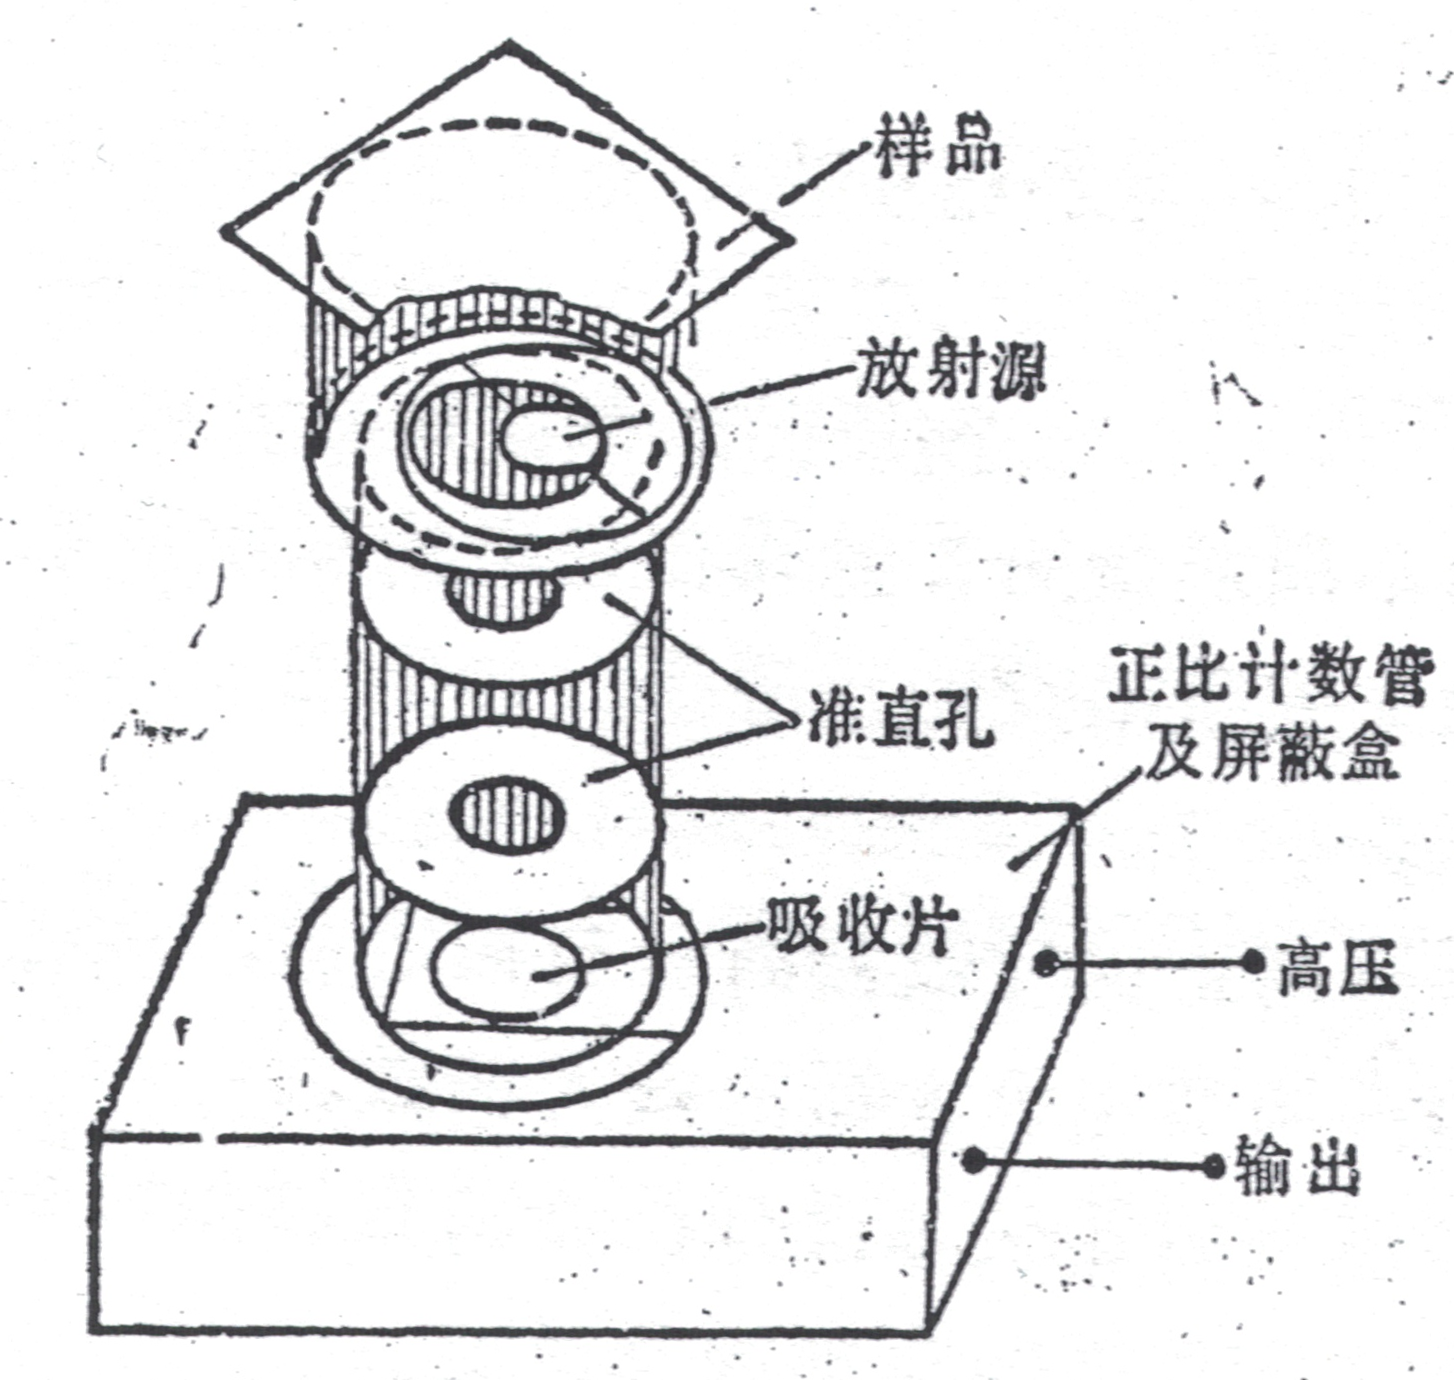
\includegraphics[width=0.45\textwidth]{yiqi.png}
\\
\xiaowu\song 图~1\begin{minipage}[t]{75mm} \quad 实验装置示意图。放射源$^{238}$Pu产生的X射线向上打到样品上,激发的X特征射线则反向进入正比计数管从而被探测产生信号。\\[-1mm]\wuhao
\end{minipage}
\end{center}

首先打开仪器,调整高压和放大倍数到合适的范围。本次实验中高压为2000V,放大倍数为209.6倍。

随后将Zn,Ge,Cr,Fe,Cu以及三个未知样品分别放到样品架上,测量其特征X谱线。得到的数据如下表所示:

 \begin{center}
\bgliu
{\bf 表~1\quad
探测到的不同材料的X射线特征的峰位以及其对应的理论能量。}\\[0.5mm]
\renewcommand{\arraystretch}{1.5}
\liuhao\song\rm
\newcolumntype{M}{>{\centering\arraybackslash}m{10mm} >{\centering\arraybackslash}m{8mm}
>{\centering\arraybackslash}m{8mm}>{\centering\arraybackslash}m{8mm}}
\begin{tabular}{M}
\specialrule{0.1em}{1pt}{1pt}

元素 &  峰道址 &  射线能量/KeV \\
\midrule
Zn &  562   &  8.638 \\
Ge &  646   &  9.885 \\
Cr &  352   &  5.414 \\
Fe &  414   &  6.403 \\
Cu &  521   &  8.047 \\
未知1   &  484   &  -  \\
未知2   &  316   &  -  \\
未知3   &  447   &  -  \\
\specialrule{0.1em}{3pt}{2pt}\\[-4mm]
\end{tabular}\\
\renewcommand{\arraystretch}{1.0}
\end{center}

可以作图拟合得到探测器系统道址和能量的对应关系,如下图所示:
\begin{center}
   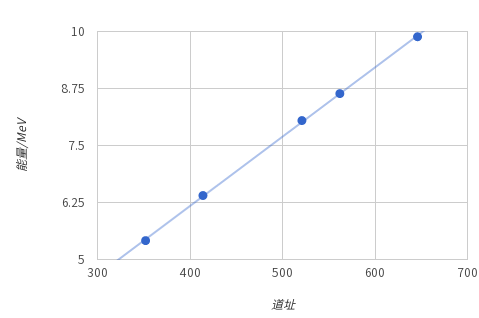
\includegraphics[width=0.45\textwidth]{1.png}
\\
\xiaowu\song 图~1\begin{minipage}[t]{75mm} \quad 探测器通道址和能量关系的标定图\\[-1mm]\wuhao
\end{minipage}
\end{center}
可以得到相应的现行关系,即:
\begin{equation}
   Energy = (0.015 \times channel + 0.0095)KeV
\end{equation}
因而得知未知样品对应的特征能量为7.355KeV,4.835KeV,6.8KeV,对应的材料为Ni, V, Co。

接下来是测定铝片对铜样品产生的特征X射线的质量吸收系数。放置不同数量的铝片(厚度均为2.15mg/cm$^2$),即可探测得到对应的能谱。选定积分范围为从477道到566道,统计测量得到的计数数目,即可计算吸收系数。 

已知$I=I_0e^{-\mu_m\rho t}$,在两边取对数之后我们可以得到 $\ln{I} = c_1 \times \rho t
+ c_2$的线性关系,其中$c_1$便是我们待测的$\mu_m$。测量得到的数据表和数据图如下:

\begin{center}
\bgliu
{\bf 表~2\quad
测量铝对X射线的吸收系数的数据表。}\\[0.5mm]
\renewcommand{\arraystretch}{1.5}
\liuhao\song\rm
\newcolumntype{M}{>{\centering\arraybackslash}m{10mm} >{\centering\arraybackslash}m{8mm}
>{\centering\arraybackslash}m{8mm}>{\centering\arraybackslash}m{8mm}}
\begin{tabular}{M}
\specialrule{0.1em}{1pt}{1pt}
厚度/$g/cm^2$ &  计数 &  测量时间/s   \\
\midrule
0  &  25814 &  600   \\
0.0043   &  38594 &  1200  \\
0.0086   &  31254 &  1200  \\
0.0129   &  24844 &  1200  \\
0.0172   &  19872 &  1200  \\
0.0215   &  15842 &  1200  \\
\specialrule{0.1em}{3pt}{2pt}\\[-4mm]
\end{tabular}\\
\renewcommand{\arraystretch}{1.0}
\end{center}
\begin{center}
   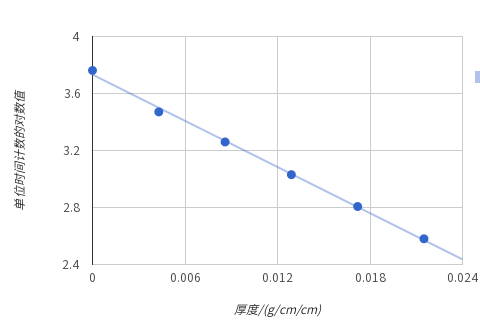
\includegraphics[width=0.45\textwidth]{2.png}
\\
\xiaowu\song 图~2\begin{minipage}[t]{75mm} \quad 测量铝对X射线的吸收系数的数据图。\\[-1mm]\wuhao
\end{minipage}
\end{center}

线性回归得到的拟合结果为:
\begin{equation}
   ln(I)=-54.0*x +3.732
\end{equation}
因而计算得到质量吸收系数$\mu_m = 54.0 cm^2/g$

最后利用$^{55}$Fe测量探测器的能量分辨率,如下图所示:
\begin{center}
   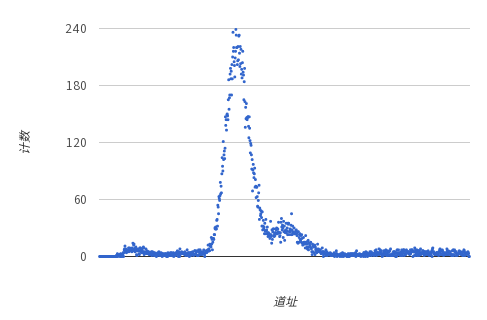
\includegraphics[width=0.45\textwidth]{3.png}
\\
\xiaowu\song 图~2\begin{minipage}[t]{75mm} \quad 测量铝对X射线的吸收系数的数据图。\\[-1mm]\wuhao
\end{minipage}
\end{center}
测量得到探测器测量Fe的峰的能量分辨率为18.3\%。

\section{结论}

本次实验通过使用正比计数器测量了不同材料在$^{238}$Pu产生的X射线的激发下发出的特征X射线,并测量推断了三个未知样品分别为Ni,V,Co。随后测量了铝对铜的特征X射线质量吸收系数为$54.0 cm^2/g$。最后利用Fe测量了该探测器的能量分辨率为18.3\%。

\section{参考文献}

\noindent
[1] Peking Unviersity, Fudan University \ Nuclear Experment
\ Nuclear Publishing House, 1989 (in Chinese)

\noindent
 (北京大学,复旦大学.\ 原子核实验\ 原子能出版社,\ 1989)

\end{multicols}

\newpage


%\section*{附录:思考题}


\clearpage
%\end{CJK*}
\end{document}

